
Amidakuji is a custom in Japan which 
allows for a pseudo-random assignment of children to prizes \cite{A23}. 
Usually done in Japanese schools, a teacher will draw $N$ vertical lines, 
hereby known as lines, where $N$ is the number of students in class. 
At the bottom of each line will be a unique prize. 
And at the top of each line will be the name of one of the students.  
The teacher will then draw 0 or more horizontal lines, hereby known as \emph{bars}, 
connecting two adjacent lines. The more bars there are the more complicated (and fun) 
the Amidakuji is. No two endpoints of two bars can be touching. Each student then traces 
their line, and whenever they encounter an end point of a bar along their line, 
they must cross the bar and continue going down the adjacent line. 
The student continues tracing down the lines and crossing bars 
until they get to the end of the ladder lottery. The prize at the bottom of the ladder lottery 
is their prize \cite{A7}. See Figure \ref{fig:aa} for an example of a ladder lottery.\par
The exact date at which Amidakuji were invented is unknown. However, the word Amidakuji has
an interesting etemology. In Japanese, Amida is the Japanese name 
for Amitabatha, the supreme Buddha of the Western Paradise. See image ---image ref---
for a picture af Amithaba. Amithaba
is a Buddha from India and there is a cult based around him. The cult 
of Amida, otherwise known as Amidism, believes that by worshiping Amithaba, they shall 
enter into the his Western Paradie. Amidism began in India in the fourth century
and made its way to China and Korea in the fifth centur, and finally  came 
to Japan in ninth century. It was in Japan, where the game Amidakuji
began. It is known as 'Ghost Legs' in China and  Ladder Lotteries in English.\par
The game Amidakuji began in Japan in the Muromachi period, which spanned from
1336 to 1573. During the Muromachi period, the game was played by having
players draw their names at the top of the lines, and at the bottom 
of the lines were pieces of paper that had the amount the players
were willing to bet. The pieces of paper were folded in the shape of 
Amithaba's halo, which is why the game is called Amidakuji. Kuji 
is the Japanese word for lottery. Hence the name of the game being 
Amidakuji.\par 
%%FUCKING LATEX.....
\begin{figure}
 \begin{center}
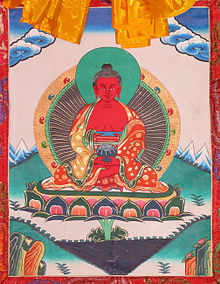
\includegraphics[scale=0.8]{220px-Buddha_Amithaba.jpg}
\captionof{figure}{A picture of Buddha Amithaba}
\end{center}
\end{figure} 

\begin{figure}[!htp]
	\begin{center}
		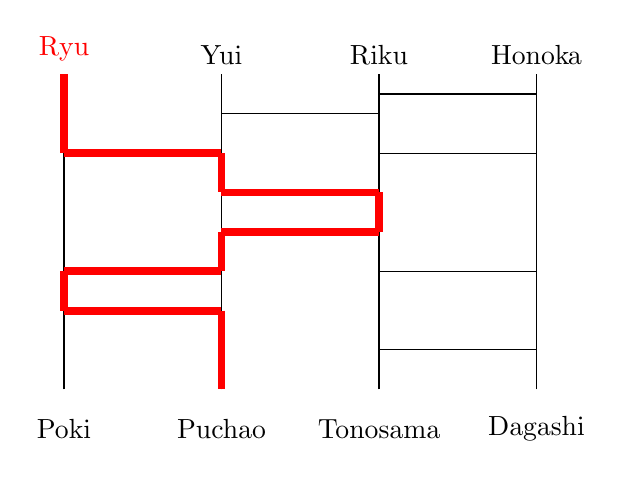
\begin{tikzpicture}
		%%Start of figure. Fig 1
			\draw(0, 0) to (0, 3); 
		
			\node at (0, -0.5){Poki};
			\draw(2, 0) to (2, 4) node[above]{Yui};
			\node at (2, -0.5){Puchao};
			\draw(4, 0) to (4, 4)node[above]{Riku};
			\node at (4, -0.5){Tonosama};
			\draw(6, 0) to (6, 4)node[above]{Honoka};
			\node at (6, -0.5){Dagashi};
			
			%bars%
		    \draw[line width=1mm, red](0, 3) to (0, 4) node[above]{Ryu};
			\draw[line width=1mm, red](0, 1) to (2, 1);
			\draw[line width=1mm, red](2, 1.5) to (2, 2);
			\draw[line width=1mm, red](0, 1)to(0, 1.5);
			\draw[line width=1mm, red](2, 1) to (2, 0);
			\draw[line width=1mm, red](0, 3) to (2, 3);
			\draw[line width=1mm, red](2, 3) to (2, 2.5);
			\draw[line width=1mm, red](4, 2) to (4, 2.5);
			\draw[line width=1mm, red](0, 1.5) to (2, 1.5);
			
			\draw[line width=1mm, red](2, 2) to (4, 2);
			\draw[line width=1mm, red](2, 2.5) to (4, 2.5);
			\draw(2, 3.5) to (4, 3.5);
			
			\draw(4, 0.5) to (6, 0.5);
			\draw(4, 3) to (6, 3);
			\draw(4, 1.5) to (6, 1.5);
			\draw(4, 3.75) to (6, 3.75);
		\end{tikzpicture}
		\caption{A ladder lottery where Ryu gets Puchao, Yui gets Dagashi, Riku gets Tonosama and Honoka gets Poki. You can see that Ryu's path is marked by red bars.}
		\label{fig:aa}

	\end{center}

\end{figure}
